% !TEX encoding = UTF-8 Unicode

\documentclass[twocolumn,10pt,a4j]{jsarticle}
\usepackage{kougai}

\title{積み上げ型教科の理解促進のための一考察}
\author{1532009 阿部 希駿  指導教員 須田 宇宙 准教授}
\date{}

\begin{document}

\maketitle

\section{はじめに}

%背景
中学,高校で学習する科目の中で数学と英語は苦手になりやすいと言われている\cite{1}.この2科目の共通点として「積み上げ型教科」である点が挙げられる.積み上げ型教科とは学習した単元を前提知識として他の単元の学習を行う教科で,本研究では前提知識となる単元を「前提単元」,前提知識を用いて学習を行う単元を「主単元」と称する.前提単元には学習目的が主単元で利用することになっているものがあり,このような単元は学習目的や実用例などがイメージがしづらく,理解の妨げになっていると考えた.
%問題点

そこで前提単元がわかりづらく,主単元がわかりやすいときに限り,「主単元の概要をあらかじめ学習することで,前提単元の理解を促進することができる」という仮説を立てた.
本研究では,講義において学生を対象とした実験を行い,この仮説を検証することを目的とする.



\section{実験の構想}

本研究では2018年後期に開講される情報数学応用の講義履修者を対象に対照実験を行う.
図\ref{fig:time}に示す順で1週目と2週目に講義を行い,3週目に小テストを行う.Aクラスでは前提単元を学習した後に主単元を学習する.それに対してBクラスではあらかじめ主単元の概要を理解することを目的に,主単元であるブロックチェーンの導入部を先に学習する.

\begin{figure}[H]
\centering
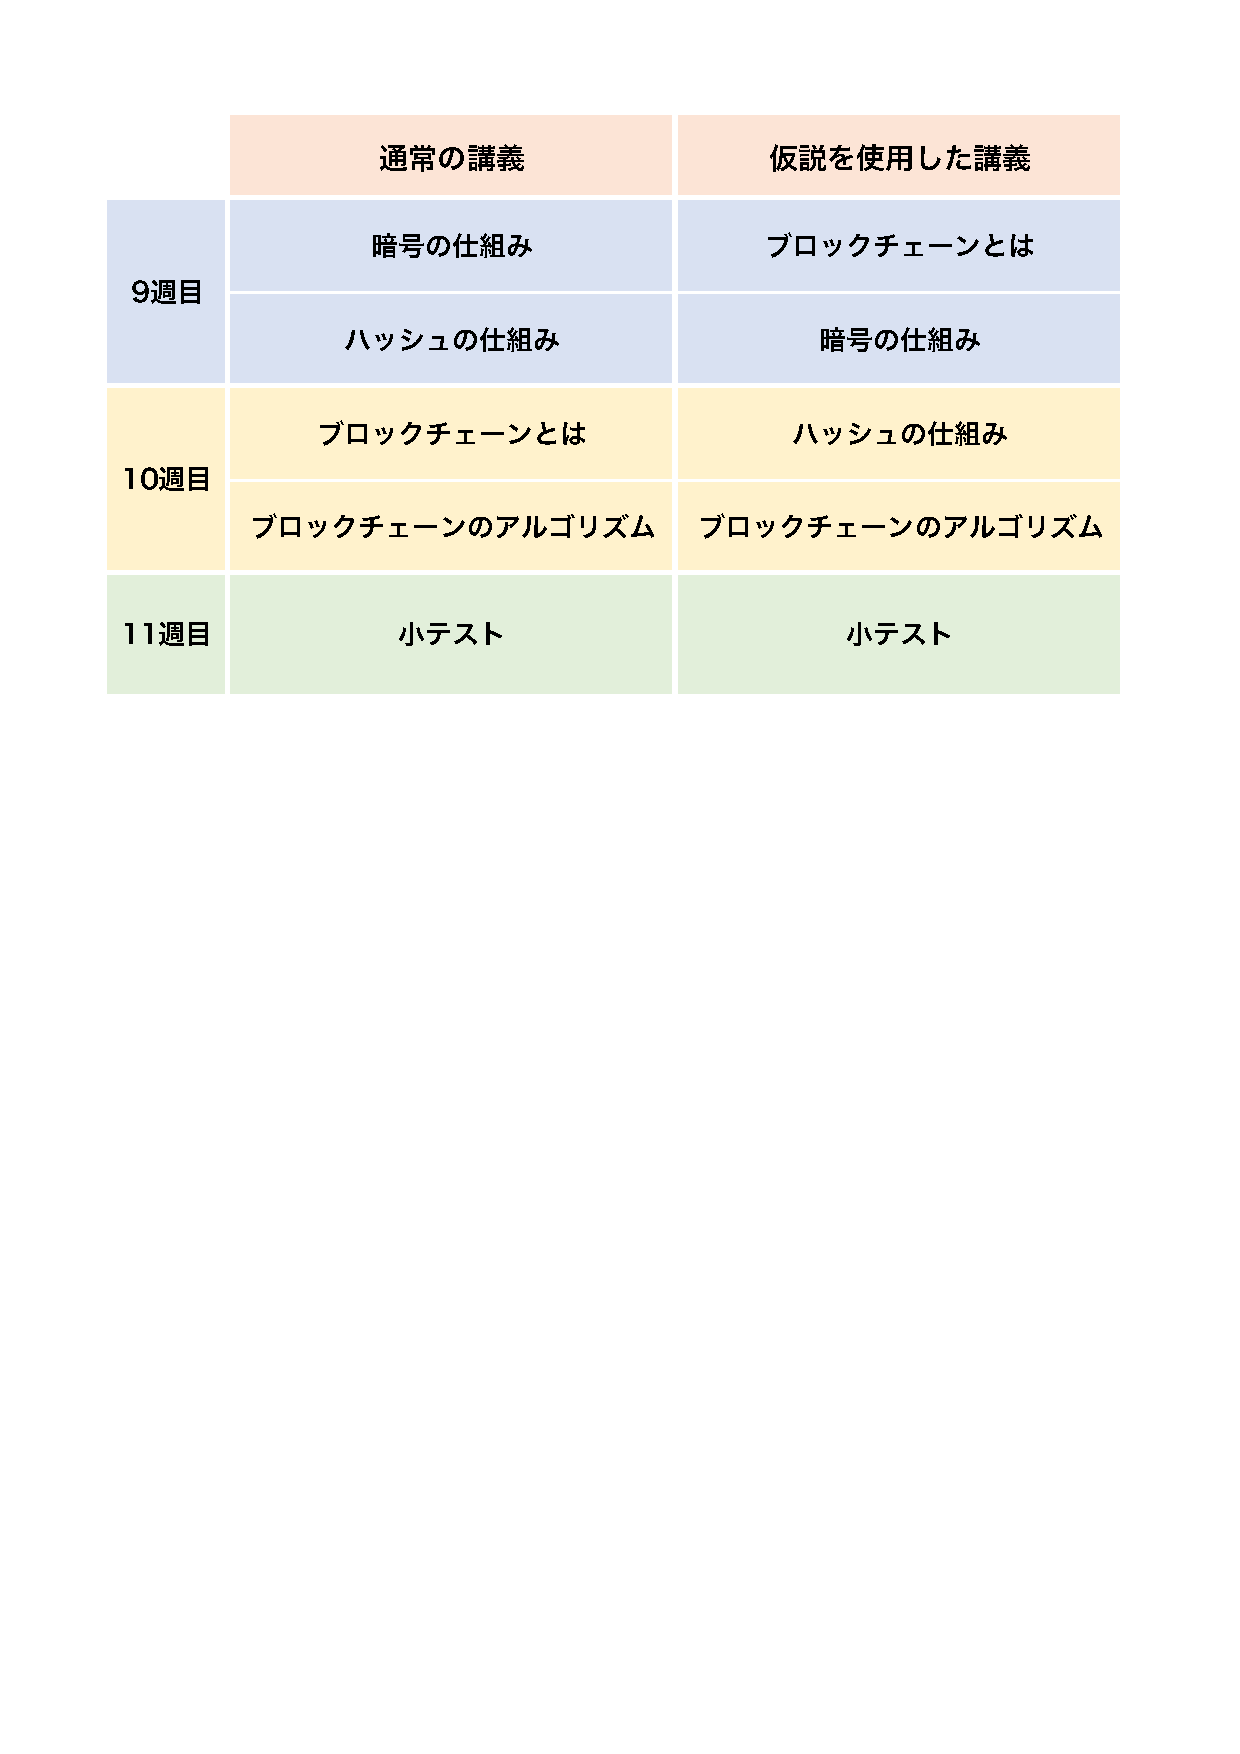
\includegraphics[mediaboxonly=/CropBox,width=8cm]{timeline.pdf}
\caption{実験で行う授業の流れ}
\label{fig:time}
\end{figure}


小テストでは以下の3項目の問題とアンケートを用意する.
\begin{itemize}
\item 暗号の仕組み
\item ハッシュと暗号の違い
\item ブロックチェーンの仕組み
\end{itemize}


「暗号の仕組み」と「ハッシュと暗号の仕組み」を前提単元,「ブロックチェーンの仕組み」を主単元とし,それぞれ5点満点とする.小テストの結果から平均点と偏差値を単元ごとに求め,元の学力差を考慮するために中間試験の偏差値を参考にする.
アンケートでは講義を受ける以前にブロックチェーンの仕組みについての知識の有無,「暗号」「ハッシュ」「ブロックチェーン」それぞれの講義内容がわかりやすかったかについて尋ねた.
小テストとアンケートの分析対象は中間試験の受験者かつブロックチェーンを講義前に学習していない学生とした.


\section{結果と考察}
各クラスの偏差値と平均点を表\ref{fig:12ank}に示す.

表\ref{fig:12ank}より前提単元,主単元ではAクラスの偏差値がわずかに高くなったが,元の学力の指標とした中間試験の偏差値との差は見られなかった.
したがって講義の順序を入れ替えても理解度は変わらないという結果になり,仮説を証明することができなかった.
そこで仮説が証明できなかった原因を表\ref{fig:12ank}やアンケート結果から以下のように考察した.


\begin{enumerate}
\item 前提単元の平均点が主単元の平均点を大きく上回ったことから問題の難易度に差があったことがわかる.講義スケジュールの関係で1週目と2週目の間に休講日があり,前半にブロックチェーンの概要を学習したBクラスの得点が下がったと考えられる.
\item アンケート結果から暗号に比べ,ハッシュとブロックチェーンの講義内容がわかりにくいと答える学生が多く見られた.このことから具体例がわかりやすい単元が主単元となっておらず,主単元の選定が不適切であったと考えられる.
\end{enumerate}

\vspace{1zh}
\begin{table}[H]
\centering
\caption{各クラスの偏差値と平均点}
\scalebox{1.1}{
\begin{tabular}{|c|c|c|c|c|}
\hline
\multicolumn{1}{|l|}{} & \multicolumn{2}{c|}{Aクラス} & \multicolumn{2}{c|}{Bクラス} \\ \cline{2-5}
                              & 偏差値 & 平均点  & 偏差値 & 平均点             \\ \hline
前提単元              & 50.4 & 3.4 /5  & 49.5 & 3.3 /5               \\ \hline
主単元                       & 51.2 & 2.5 /5       & 48.7 & 2.1 /5                           \\ \hline
中間試験                       &50.6  & 29.4 /50 & 49.3 &     28.0 /50                  \\ \hline
\end{tabular}
}
\label{fig:12ank}
\end{table}




\section{おわりに}
本研究では積み上げ型教科の理解度を上げる仮説を立て,実験を行なった.今回の実験では仮説が正しいと証明することができなかったが,実験の改善点が見つかったため,今後はさらなる実験を行い検証することが望まれる.

\begin{thebibliography}{99}
\bibitem{1}
ベネッセ教育情報サイト:“教科学習が不得意と感じている高校生が9割!そのほとんどが英語と数学に偏るのにはある理由が”, \url{https://www.benesse.jp/kyouiku/201603/20160329-3.html}, (参照 2018-8-14)
\end{thebibliography}

\end{document}